\documentclass[ee577b,acmnow]{acmtrans2m}

\usepackage{graphicx}
%\usepackage[margin=1.0in,vmargin={30pt,2cm},nohead]{geometry}
%\usepackage{amsmath, amsthm,  amsfonts, amscd}
\usepackage{url}
%\usepackage{cite}
%\usepackage{fancyhdr}

%\acmVolume{1}
%\acmNumber{1}
\acmYear{07}
\acmMonth{October 10,}

\newtheorem{theorem}{Theorem}[section]
\newtheorem{conjecture}[theorem]{Conjecture}
\newtheorem{corollary}[theorem]{Corollary}
\newtheorem{proposition}[theorem]{Proposition}
\newtheorem{lemma}[theorem]{Lemma}
\newdef{definition}[theorem]{Definition}
\newdef{remark}[theorem]{Remark}


           
\markboth{EE 577B Fall 2007: Extra Credit Homework \#1}
{EE 577B Fall 2007: Extra Credit Homework \#1}

\title{EE 577B Fall 2007: Extra Credit Homework \#1}
            
\author{Zhiyang Ong\\
Ming Hsieh Department of Electrical Engineering,\\
Viterbi School of Engineering,\\
University of Southern California
}
            
\begin{abstract} 
Synthesizable behavorial RTL models for the encoder and decoder
of the (15,11,3) Hamming code were developed in Verilog. They
were synthesized into Verilog netlists, and simulation-based
verification were used to check the behavioral models and the
synthesized Verilog netlists.
\end{abstract}
            
\category{VLSI}{Digital IC Design}{Communication Electronics}
            
\terms{Error Correction and Detection, Logic Synthesis, Functional
Verification} 
            
\keywords{Error-Correcting Code, Parity-Check Matrix, Generator Matrix,
Decoder,Encoder}
            
\begin{document}
\setcounter{page}{1}
            

            
\maketitle

\section{Introduction}

The encoder and decoder of the (15,11,3) Hamming code \cite{Weste05} were
developed in Verilog, using synthesizable behavorial RTL models.
They were verified using circuit simulation. Subsequently,
logic synthesis was performed on these models of the encoder
and the decoder. The resultant synthesized Verilog netlists
were verified via simulation again.

Section 1 describes the generation of the generator and parity-check
matrices used for creating the encoder and the error-correcting decoder.
Next, Section 2 indicates the implementation of the encoder and decoder as
synthesizable behavorial RTL models in Verilog. Subseuqently, Section 4
describes how they fit into a pipelined communications channel, which
is simulated. Following that is Section 5 which describes the results
from performing logic synthesis on the behavioral models, and Section
6 which describes how the simulation waveforms differ in the synthesized
Verilog netlists from the behavioral models. Finally, Section 7 draws
conclusion on this brief report.

\section{Generator matrix G and Parity Check Matrix H}

In Table \ref{bitscbp}, the relationship between data bits, $B_{i}$, and parity bits, $P_{i}$, with the encoded data bits, $C_{i}$ is given. This is used to form the relationships between data bits, $B_{i}$, and parity bits, $P_{i}$, as indicated below.\\
\ \\
P1 = B1 + B2 + B4 + B5 + B7 + B9 + B11\\
P2 = B1 + B3 + B4 + B6 + B7 + B10 + B11\\
P3 = B2 + B3 + B4 + B8 + B9 + B10 + B11\\
P4 = B5 + B6 + B7 + B8 + B9 + B10 + B11\\

\begin{table}
\caption{Table representing the relationship between data bits, $B_{i}$, and parity bits, $P_{i}$, with the encoded data bits, $C_{i}$}
\label{bitscbp}
\begin{tabular}{|c|c|c|c|c|c|c|c|c|c|c|c|c|c|c|}
\hline
C1 & C2 & C3 & C4 & C5 & C6 & C7 & C8 & C9 & C10 & C11 & C12 & C13 & C14 & C15\\
\hline
P1 & P2 & B1 & P3 & B2 & B3 & B4 & P4 & B5 & B6 & B7 & B8 & B9 & B10 & B11\\
\hline
\end{tabular}
\end{table}
\ \\
The parity check matrix H and the generator matrix G for the $m = 4$ Hamming code with $d_{min} = 3$ is given as follows: \\
\ \\
$H = \left [ \begin{array}{ccccccccccccccc}
1 & 0 & 1 & 0 & 1 & 0 & 1 & 0 & 1 & 0 & 1 & 0 & 1 & 0 & 1 \\
0 & 1 & 1 & 0 & 0 & 1 & 1 & 0 & 0 & 1 & 1 & 0 & 0 & 1 & 1 \\
0 & 0 & 0 & 1 & 1 & 1 & 1 & 0 & 0 & 0 & 0 & 1 & 1 & 1 & 1 \\
0 & 0 & 0 & 0 & 0 & 0 & 0 & 1 & 1 & 1 & 1 & 1 & 1 & 1 & 1 \\
\end{array} \right ] $\\
\ \\
\ \\
\ \\
$G = \left [ \begin{array}{ccccccccccccccc}
1 & 1 & 1 & 0 & 0 & 0 & 0 & 0 & 0 & 0 & 0 & 0 & 0 & 0 & 0 \\
1 & 0 & 0 & 1 & 1 & 0 & 0 & 0 & 0 & 0 & 0 & 0 & 0 & 0 & 0 \\
0 & 1 & 0 & 1 & 0 & 1 & 0 & 0 & 0 & 0 & 0 & 0 & 0 & 0 & 0 \\
1 & 1 & 0 & 1 & 0 & 0 & 1 & 0 & 0 & 0 & 0 & 0 & 0 & 0 & 0 \\
1 & 0 & 0 & 0 & 0 & 0 & 0 & 1 & 1 & 0 & 0 & 0 & 0 & 0 & 0 \\
0 & 1 & 0 & 0 & 0 & 0 & 0 & 1 & 0 & 1 & 0 & 0 & 0 & 0 & 0 \\
1 & 1 & 0 & 0 & 0 & 0 & 0 & 1 & 0 & 0 & 1 & 0 & 0 & 0 & 0 \\
0 & 0 & 0 & 1 & 0 & 0 & 0 & 1 & 0 & 0 & 0 & 1 & 0 & 0 & 0 \\
1 & 0 & 0 & 1 & 0 & 0 & 0 & 1 & 0 & 0 & 0 & 0 & 1 & 0 & 0 \\
0 & 1 & 0 & 1 & 0 & 0 & 0 & 1 & 0 & 0 & 0 & 0 & 0 & 1 & 0 \\
1 & 1 & 0 & 1 & 0 & 0 & 0 & 1 & 0 & 0 & 0 & 0 & 0 & 0 & 1 \\
\end{array} \right ] $\\
\ \\
\ \\
\ \\

\section{Implementation of Encoder and Decoder modules in Verilog}
The encoder and decoder modules for encoding and decoding using linear block codes, (15,11,3) Hamming code, are implemented in Verilog, using behavioral RTL design style. The listings for the encoder, single-bit error-correcting decoder, and their testbenches are provided as attachments at the end of this report.

\hspace{-2cm}\begin{figure}
\begin{center}
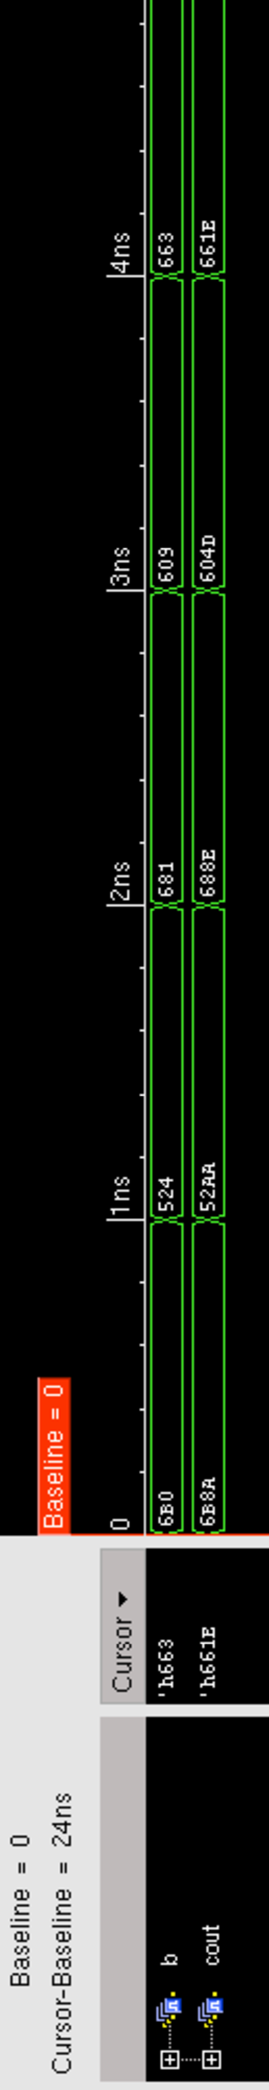
\includegraphics[height=18.5cm]{preenc}
\caption{Simulation Waveforms for the pre-synthesized Behavioral RTL for the Hamming Encoder.}
\label{preencoder}
\end{center}
\end{figure}

\hspace{-2cm}\begin{figure}
\begin{center}
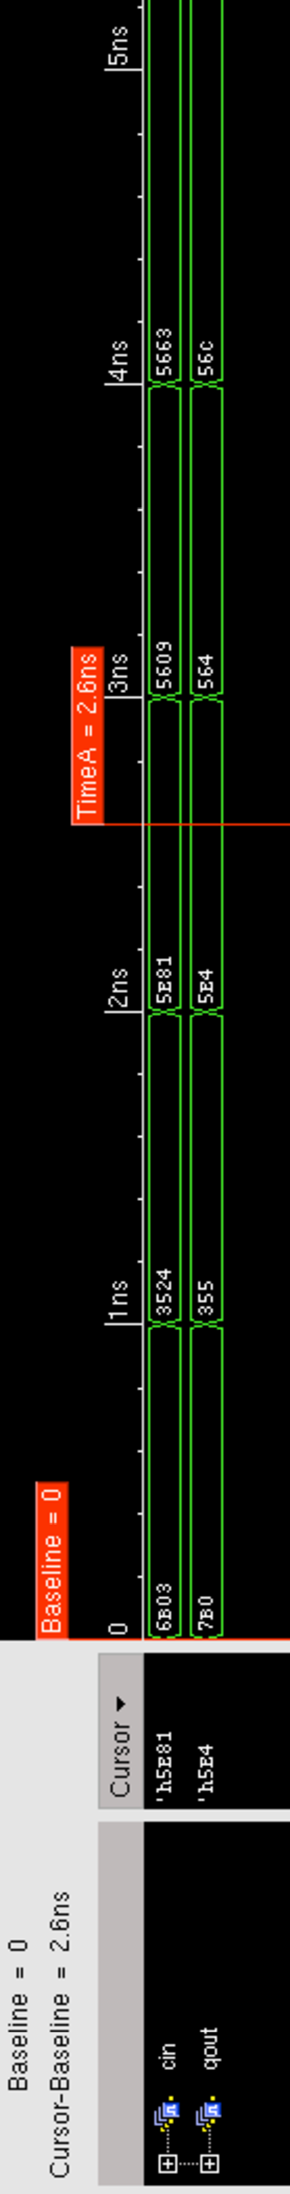
\includegraphics[height=18.5cm]{predec}
\caption{Simulation Waveforms for the pre-synthesized Behavioral RTL for the Error-Correcting Hamming Decoder.}
\label{predecoder}
\end{center}
\end{figure}

Figure \ref{preencoder} shows the simulation waveforms for the
pre-synthesized behavioral RTL for the Hamming encoder, while
Figure \ref{predecoder} shows the simulation waveforms for the
pre-synthesized behavioral RTL for the error-correcting Hamming
decoder.


\section{Development of the Testbench that Models a Communications Channel}
The testbench for a communications channel with three pipeline stages was developed; see Figure \ref{commch}. The first stage contains the Hamming encoder, while the last stage contains the error-correcting Hamming decoder and a parity-stripper module. The parity-stripper module extracts the parity bits from the encoded data bits, which may be corrupted, transmitted through the communications channel. This results in producing the data bits (qx[10:0]), which may be corrupted, at its output. 

The output of the parity-stripper module (qx[10:0]) is compared with that of the error-correcting Hamming decoder (q[10:0]), and the original data bits (rb[10:0]) that has been passed along in the communications channel. The output of the error-correcting Hamming decoder (q[10:0]) should match the original data bits (b[10:0]). If the encoded data bits are corrupted in the communications channel with a single-bit error, the error-correcting Hamming decoder should have detected it, and corrected it. Else, if more than one-bit errors are detected, errors will go uncorrected. Finally, comparing qx[10:0] with q[10:0] and rb[10:0] allows us to determine which data bits are corrupted with errors in the communications channel, and if such errors are corrected.

The second stage consist of a 4-to-16 bit decoder and a 15-bit XOR gate to model. The 4-to-16 bit decoder is used to create a 16-bit random number (err[15:1]) from a 4-bit random number (e[3:0]) that is used to represent the error signal, or noise, that is used to corrupt data bits in the communications channel. The 15-bit XOR gate is used to corrupt the encoded data bits (r\_c[14:0]) with errors (err[15:1]) in the second stage of the communications channel. This models how data can get corrupted during transmission in a communications channel.

\begin{figure}
%\vspace{-2.7cm}
%\centering
%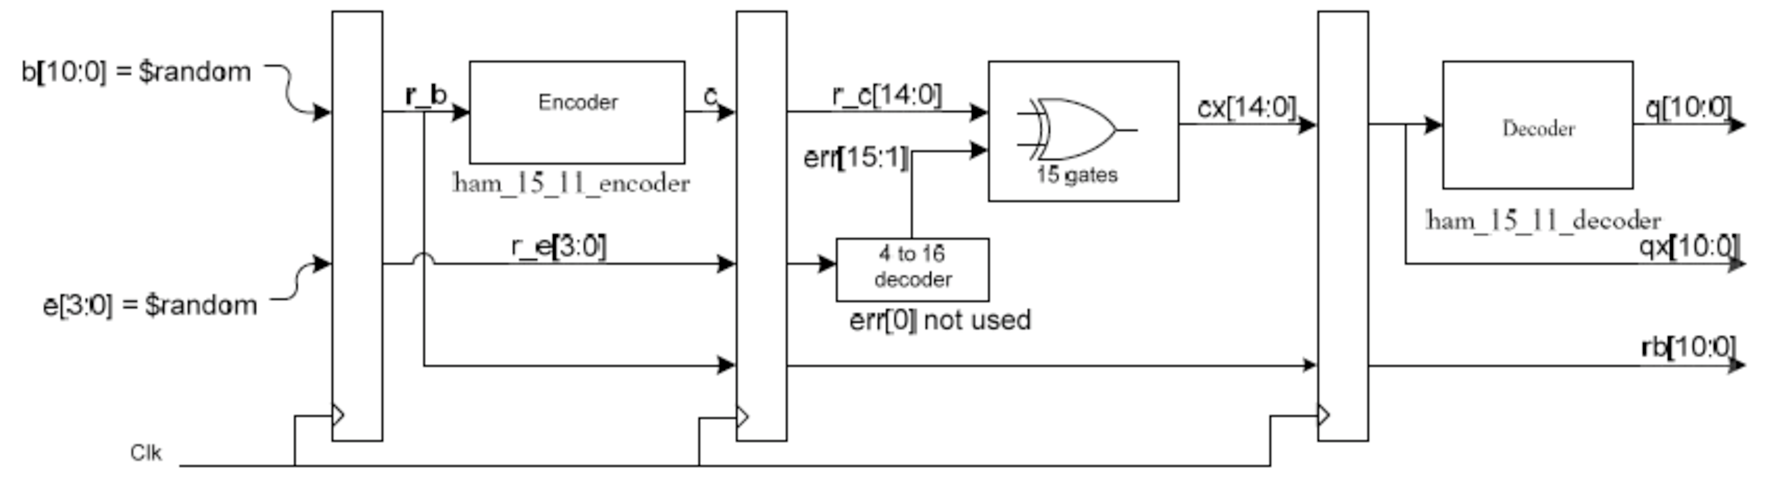
\includegraphics[width=3.5cm,height=3.5cm]{commschannel}
\begin{center}
%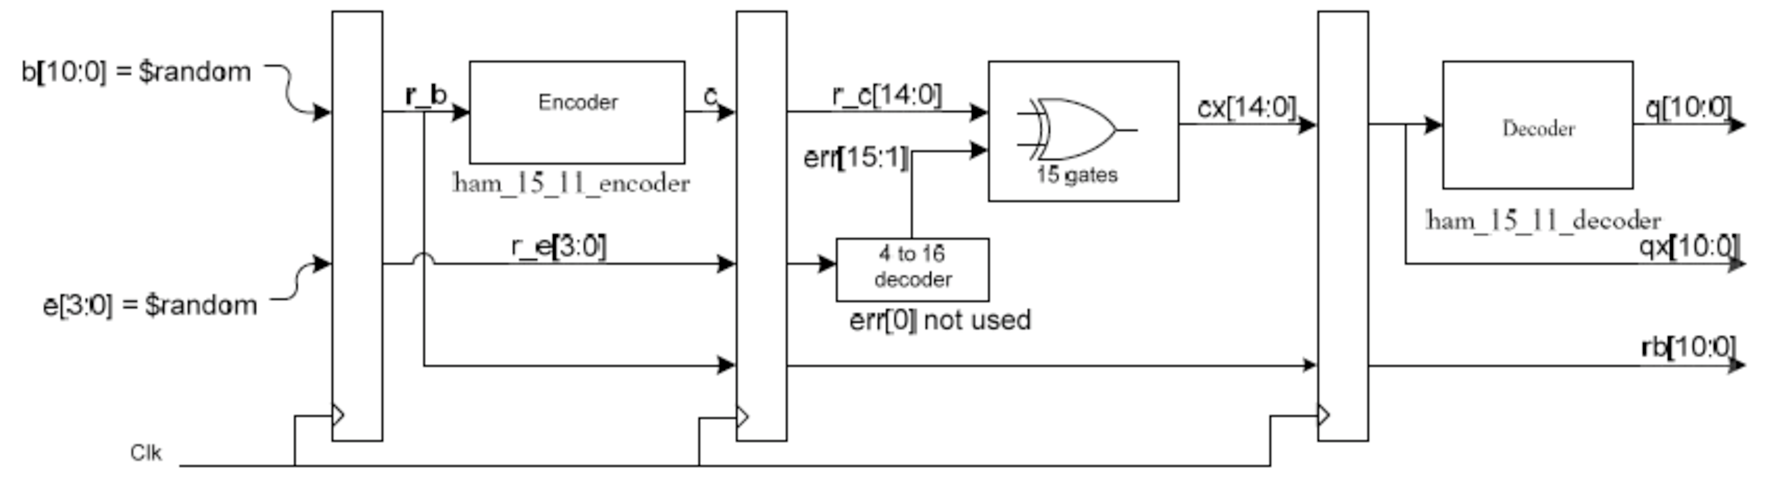
\includegraphics[width=7.5cm,height=4.0cm]{commschannel}
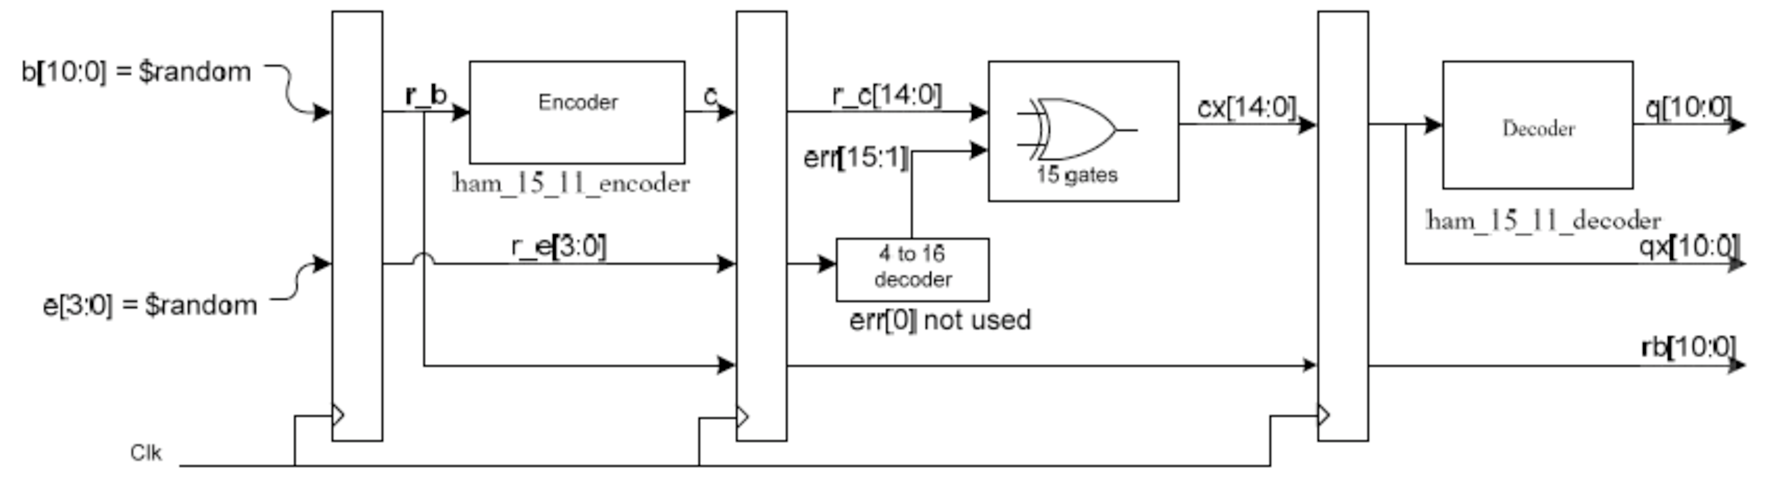
\includegraphics[width=12cm]{commschannel}
\caption{Schematic modeling a communications channel.}
\label{commch}
\end{center}
\end{figure}


Figure \ref{predecoder4to16} shows the
simulation waveforms for the behavioral RTL for the 4-to-16 bit
decoder. Lastly, Figure \ref{pref} and Figure \ref{pref1} indicate
the simulation waveforms for the pipelined communications
channel. The former shows all the signals in the three-stage
pipeline, while the latter shows only the input and output signals
of that pipeline. It is noted that the simulation of behavioral
RTL models do not use information pertinent to the interconnect
and device characteristics, and parasitics to capture the delay
through the digital logic. That is, these simulations are
performed on ideal logic components, and cannot capture delays
affecting the logic of the design.





\hspace{-2cm}\begin{figure}
\begin{center}
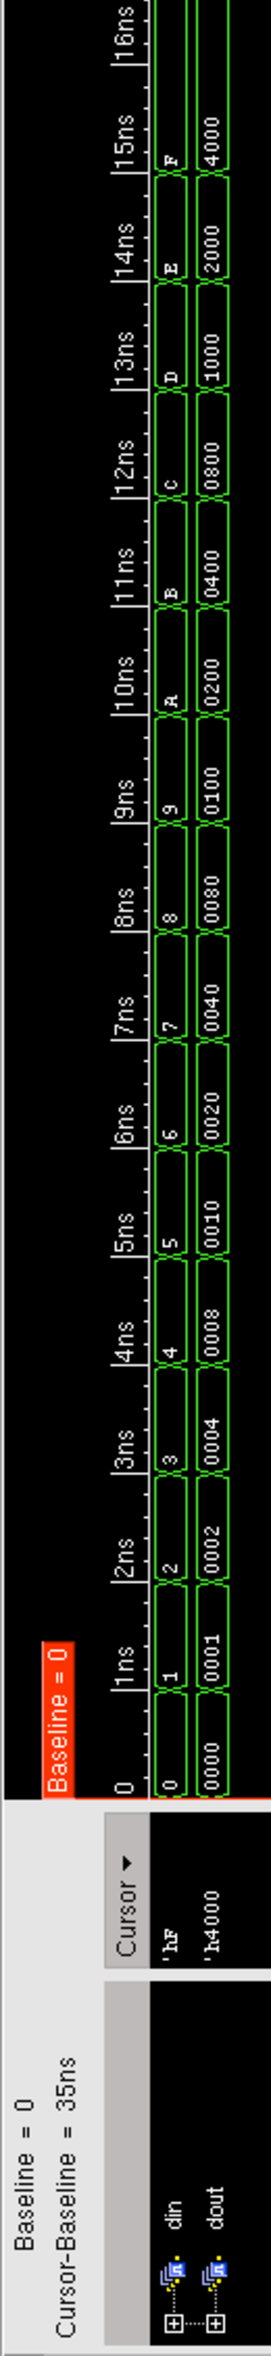
\includegraphics[height=18.5cm]{predec4to16}
\caption{Simulation Waveforms for the Behavioral RTL for the 4-to-16 bit Decoder.}
\label{predecoder4to16}
\end{center}
\end{figure}

\hspace{-2cm}\begin{figure}
\begin{center}
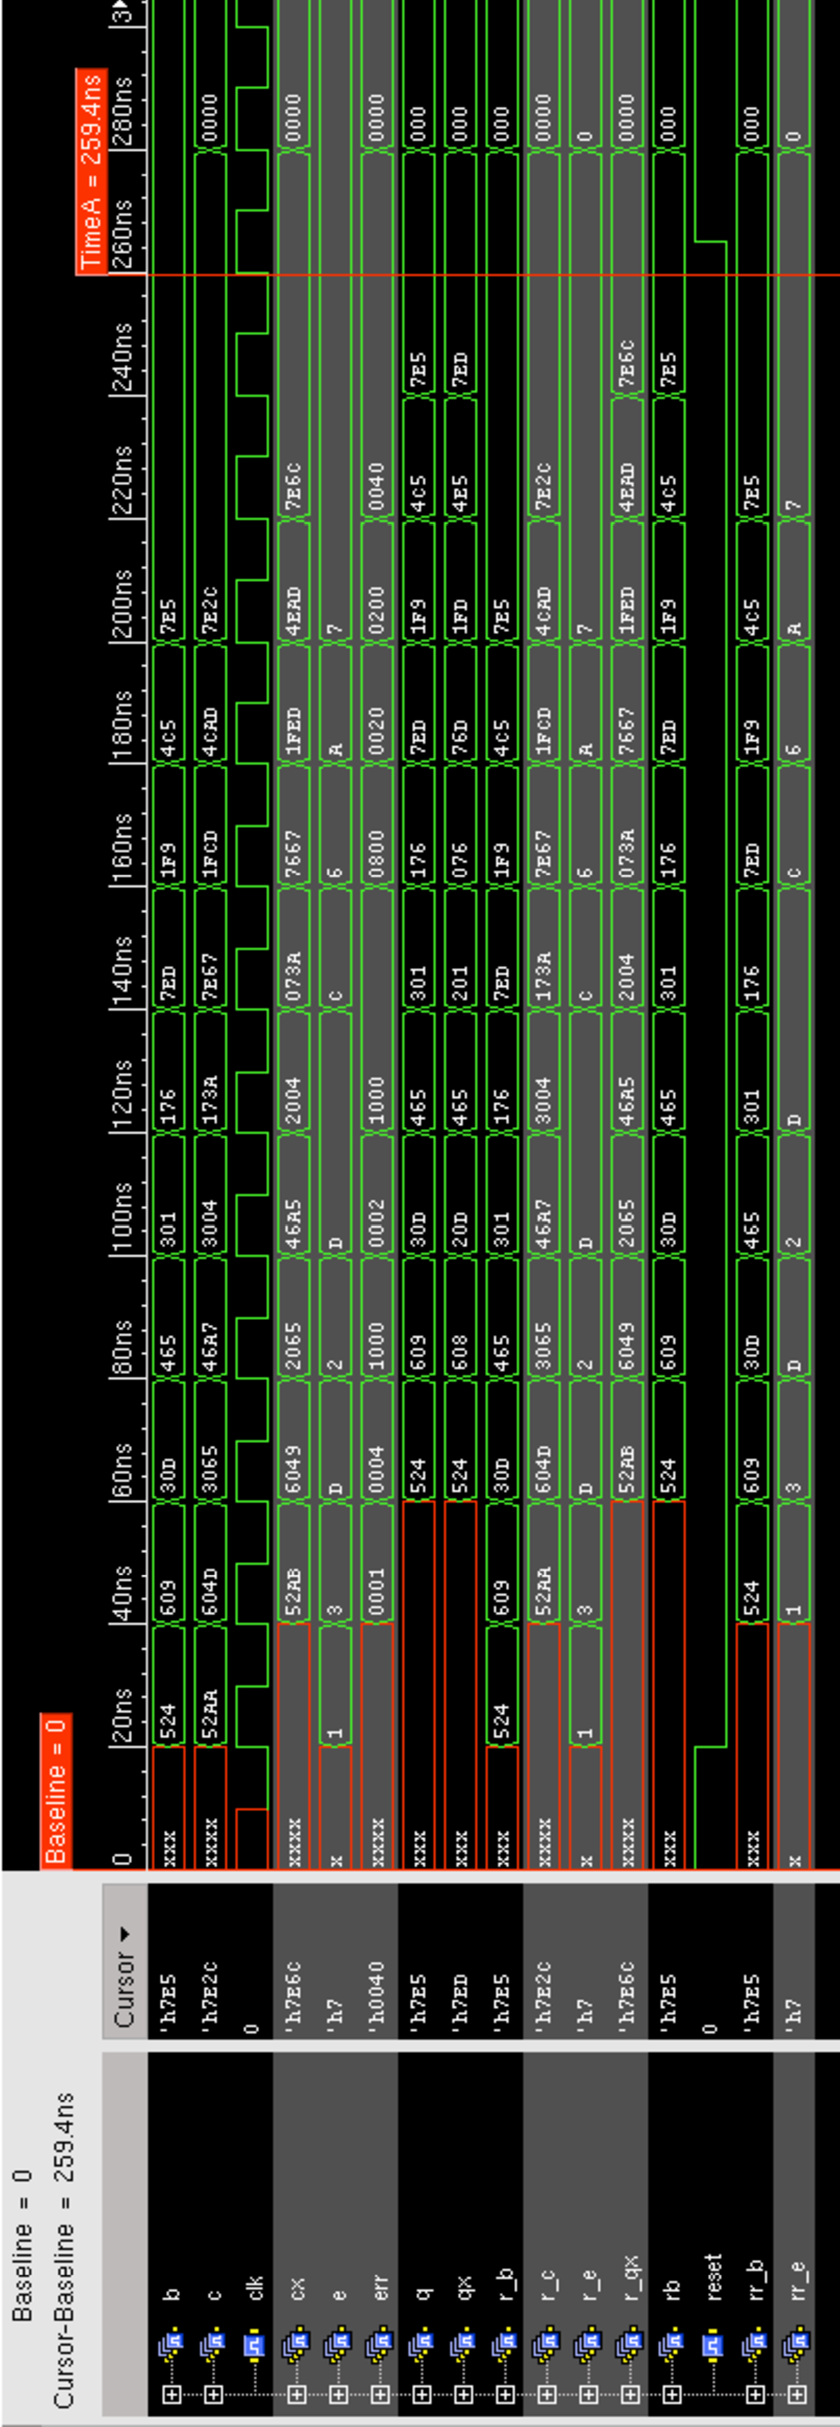
\includegraphics[height=18.5cm]{prefinal}
\caption{Simulation Waveforms for the Communications Channel.}
\label{pref}
\end{center}
\end{figure}

\hspace{-2cm}\begin{figure}
\begin{center}
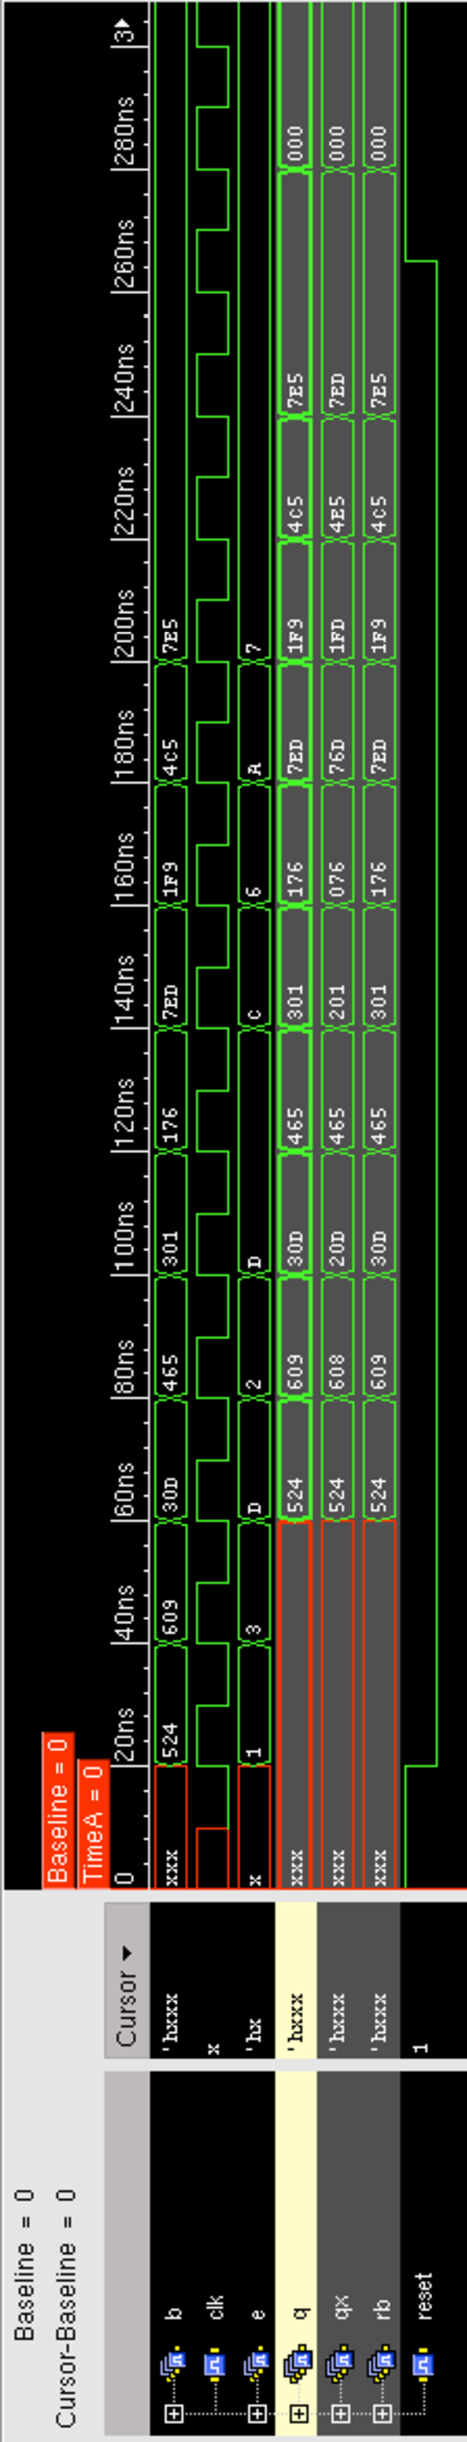
\includegraphics[height=18.5cm]{prefinal1}
\caption{Zoomed-in Display of Input and Output Simulation Waveforms for the Communications Channel.}
\label{pref1}
\end{center}
\end{figure}

\section{Logic Synthesis of Hamming Encoder and Decoder}

The area and timing reports from performing logic synthesis on
the Hamming encoder and decoder are found in the attachment. The
total area for the Hamming decoder is 3041 ${\rm units^2}$, while
its delay through its critical path(s) is 2.60 units. Its total
dynamic power consumption is 6.0982 mW, while its cell leakage
power is 6.6074 nW.

Hamming encoder has a total area of 1008 ${\rm units^2}$, while
its delay through its critical path(s) is 0.67 units. Its total
dynamic power consumption is 2.0195 mW, while its cell leakage
power is 2.9028 nW.

\section{Simulation of Synthesized Hamming Encoder and Decoder}

Figure \ref{postencoder} shows the simulation waveforms for the
synthesized Hamming encoder, while Figure \ref{postdecoder} shows
the simulation waveforms for the synthesized error-correcting
Hamming encoder.

The author notes that the simulation of the synthesized Verilog
netlists uses information pertinent to the interconnect
and device characteristics, and parasitics to capture the delay
through the digital logic. These information are provided from
the SDF files, and the technology library used for logic
synthesis. That, these simulations are performed on realistic
logic components, and can capture delays affecting the logic
of the design. For example, the correct values for the encoder
appear after a significant time delay since the encoder and the
decoder has different paths with various delays. Hence, the
values from the input may propagate to the output on certain
paths faster than other paths. Consequently, the output values
are incorrect until the values have propagated from the inputs
to the outputs on the critical path.

\section{Conclusion}

Synthesizable behavorial RTL models for the encoder and decoder
of the (15,11,3) Hamming code were developed in Verilog. They
were verified using circuit simulation. Subsequently, the
encoder and the decoder underwent logic synthesis, and were
verified via simulation again.

\hspace{-2cm}\begin{figure}
\begin{center}
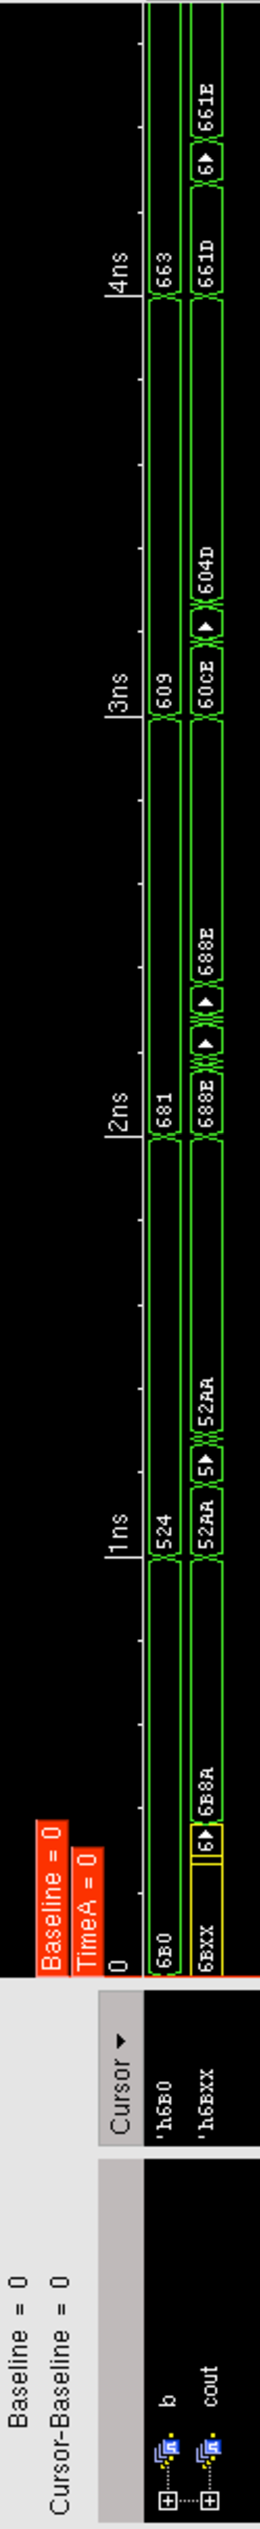
\includegraphics[height=18.5cm]{postenc}
\caption{Simulation Waveforms for the Synthesized Hamming Encoder.}
\label{postencoder}
\end{center}
\end{figure}

\hspace{-2cm}\begin{figure}
\begin{center}
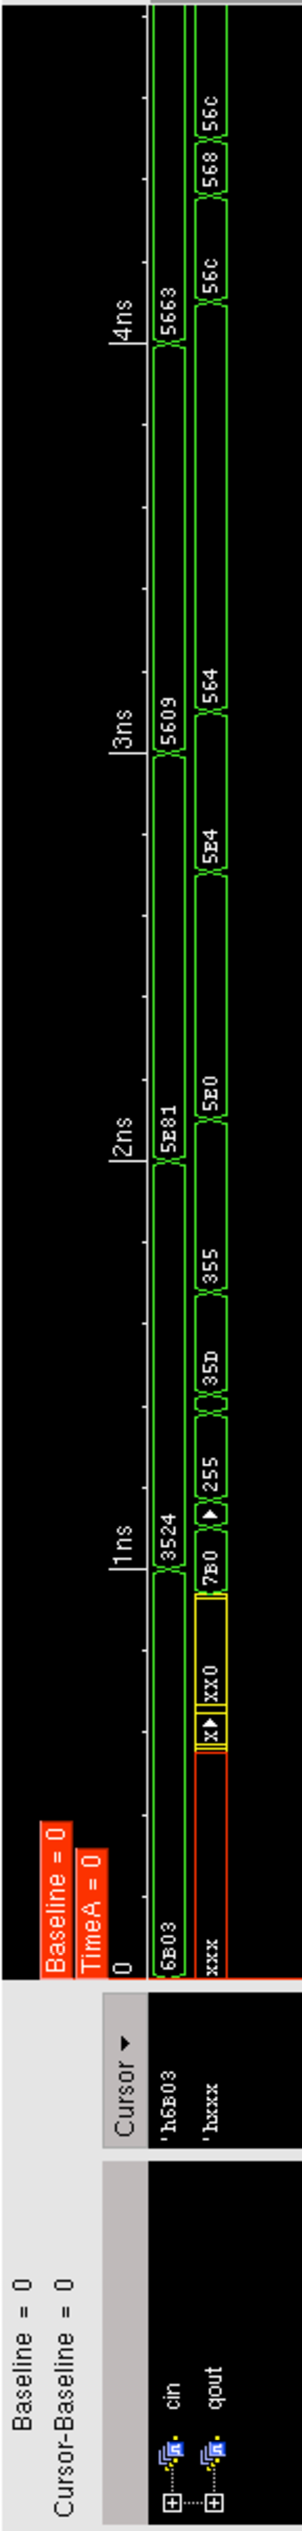
\includegraphics[height=18.5cm]{postdec}
\caption{Simulation Waveforms for the Synthesized Error-Correcting Hamming Decoder.}
\label{postdecoder}
\end{center}
\end{figure}

%This is great \cite{Weste05,Rabaey03,Kang03,Sutherland99}.

%\begin{acks}
%We thank Prof. Rashed Z. Bhatti for teaching us about SRAM design.
% Also, we express gratitude to the following teaching assistants for
% their advice and help: Ehsan Pakbazbia, Jae Chul Cha, Mahta Haghi,
% and Youngki Choe. In addition, we appreciate the graders Hwisung
% Jung and Bhavna Chopra for spending their time to grade our work.
%\end{acks}

\bibliographystyle{acmtrans}
%\bibliography{references.bib}
%\bibliographystyle{plain}
%%%%%%%%%%%%%%%%%%%%%%%%%%%%%\bibliographystyle{unsrt}
\bibliography{references}
\begin{received}
Submitted November 19, 2007, 1200 hrs
\end{received}
\end{document}


